%% Graphical Abstract (vector). Compile on Overleaf or a full TeX install.
%% Produces a single tightly-cropped image; export to PDF or PNG as the journal requires.
\documentclass[border=12pt]{standalone}
\usepackage{tikz}
\usepackage{helvet}
\renewcommand{\familydefault}{\sfdefault}
\usetikzlibrary{arrows.meta,positioning,fit,backgrounds}

\begin{document}
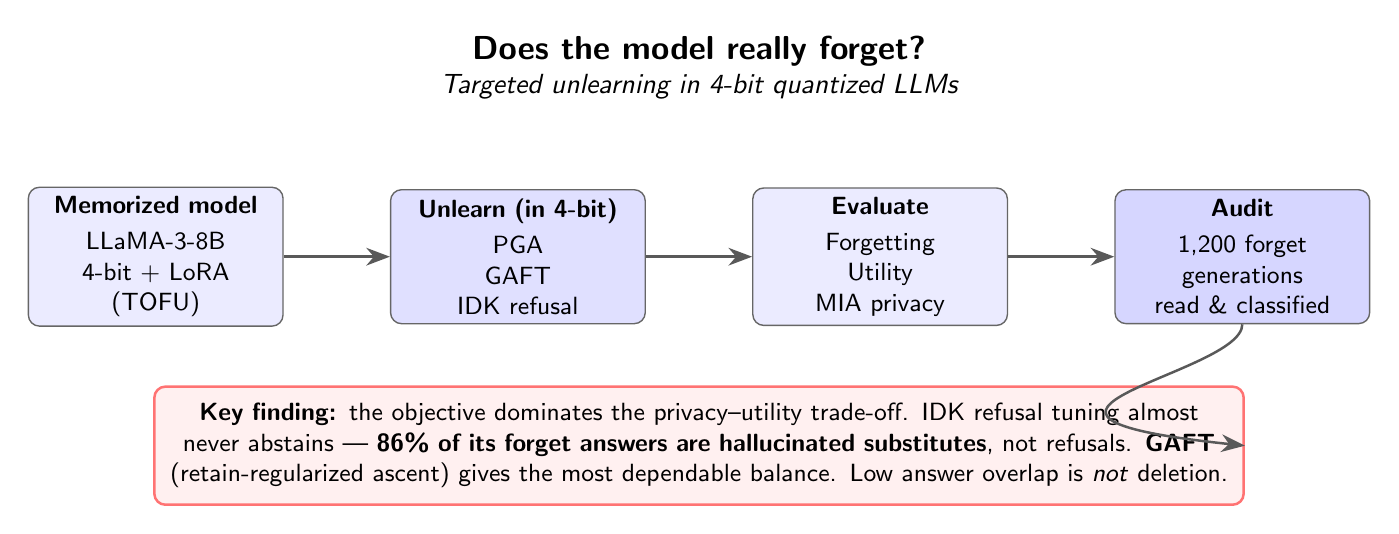
\begin{tikzpicture}[
  font=\small,
  >={Stealth[length=3mm]},
  stage/.style={rectangle, rounded corners=4pt, draw=black!60, line width=0.5pt,
                text width=3.0cm, minimum height=1.7cm, align=center, fill=blue!8},
  finding/.style={rectangle, rounded corners=4pt, draw=red!55, line width=0.9pt,
                  text width=13.6cm, minimum height=1.5cm, align=center, fill=red!6},
  arr/.style={->, line width=0.9pt, draw=black!65}
]

% Title
\node[align=center] (title) at (6.9,2.4)
  {\bfseries\large Does the model really forget?\\[1pt]
   \normalsize\itshape Targeted unlearning in 4-bit quantized LLMs};

% Pipeline stages
\node[stage] (m1) at (0,0)
  {\textbf{Memorized model}\\[2pt] LLaMA-3-8B\\ 4-bit + LoRA\\ (TOFU)};
\node[stage, fill=blue!12] (m2) at (4.6,0)
  {\textbf{Unlearn (in 4-bit)}\\[2pt] PGA\\ GAFT\\ IDK refusal};
\node[stage, fill=blue!8] (m3) at (9.2,0)
  {\textbf{Evaluate}\\[2pt] Forgetting\\ Utility\\ MIA privacy};
\node[stage, fill=blue!16] (m4) at (13.8,0)
  {\textbf{Audit}\\[2pt] 1,200 forget\\ generations\\ read \& classified};

\draw[arr] (m1) -- (m2);
\draw[arr] (m2) -- (m3);
\draw[arr] (m3) -- (m4);

% Finding box
\node[finding] (f) at (6.9,-2.4)
  {\textbf{Key finding:} the objective dominates the privacy--utility trade-off.
   IDK refusal tuning almost never abstains --- \textbf{86\% of its forget answers are
   hallucinated substitutes}, not refusals. \textbf{GAFT} (retain-regularized ascent)
   gives the most dependable balance. Low answer overlap is \emph{not} deletion.};

\draw[arr] (m4.south) .. controls (13.8,-1.5) and (10,-2.0) .. (f.east);

\end{tikzpicture}
\end{document}
